\label{sec:IF_SBND}
The SBND experiment is designed to build upon the many years of LArTPC R$\&$D and serve as a test-bed for the future long baseline neutrino experiment. SBND's design is to construct a membrane cryostat in a new on experiment hall located 110 meters from the BNB target. The cryostat will house the full TPC consisting of one central cathode plane assembly (CPA) and four anode plane assemblies (APAs) which will have three wire planes with three millimetre spacing (similar to the ICARUS design) and the first two induction planes oriented at $\pm 30^{\circ}$ to the beam axis and the final plane oriented vertically. SBND will be a 5.0~m~$\times$~4.0~m~$\times$~4.0~m (l$\times$w$\times$h) TPC with 112 tons of active volume. SBND will also have a light detection system based on a hybrid of the ICARUS cryogenic PMT's and the proposed DUNE light-guide with silicon photomultiplier (SiPMs) on the end. This light detection system will be embedded behind the APA structure on both sides of the TPC. 

%\begin{figure}[htb]
%\centering
%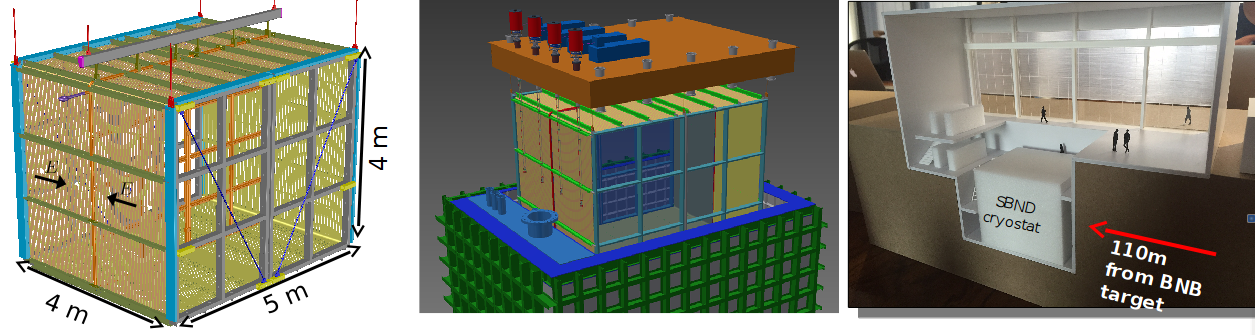
\includegraphics[width=0.75\textwidth]{images/sbnd.png}
%\caption[]{Conceptual design of the SBND TPC, cryostat, and detector hall.}
%\label{fig:sbnd}
%\end{figure}

One new unique aspect of the SBND detector will be the inclusion of the entire front end readout chain being moved into the liquid argon. The front end electronics are composed of 16-channel analogue front end ASIC which provides amplification and shaping, a 16 channel analogue to digital converter ASIC which provides digitization, buffering, and multiplexing as well as a cold FPGA which provides second multiplexing and voltage regulation. This technical improvement in readout electronics will provide improved signal-to-noise as well as allow for the development of an efficient zero-suppression scheme implemented in the FPGA to greatly reduce the total data volume. Many bench tests of the readout electronics have been performed and shows excellent performance, however a full integration test with an operating TPC has not been successfully performed (given the many problems seen by the 35ton prototype) and serves as an absolutely necessary service task the UTA group is planning to spearhead. 

%%%%%%%%%%%%%%%%%%%%%%%%%%%%%%%%%%%%%%%%%%%%%%%%%%%%%%%%%%%%%%%%%%%%%
\subsection{Cold Electronics Teststand}\label{sec:SBNDTeststand}
%%%%%%%%%%%%%%%%%%%%%%%%%%%%%%%%%%%%%%%%%%%%%%%%%%%%%%%%%%%%%%%%%%%%%
Figure \ref{fig:teststand} shows a schematic of what this test-stand would look like utilizing the ``Blanche'' cryostat currently installed at the Proton Assembly Building (PAB)at Fermilab. This cryostat is engineered to have delivered purified liquid argon into the cryostat as well as circulate, re-condense, and purify boil-off argon. A duplicate of this cryostat is currently being built and will be delivered in late 2016 to UTA. This cryostat will work in conjunction with the liquid argon purification system currently in operation at UTA. This system is built using start-up funds from PI Asaadi and will allow UTA to play an important role in the ability to do detector R$\&$D in the coming years. 

\begin{figure}[htb]
\centering
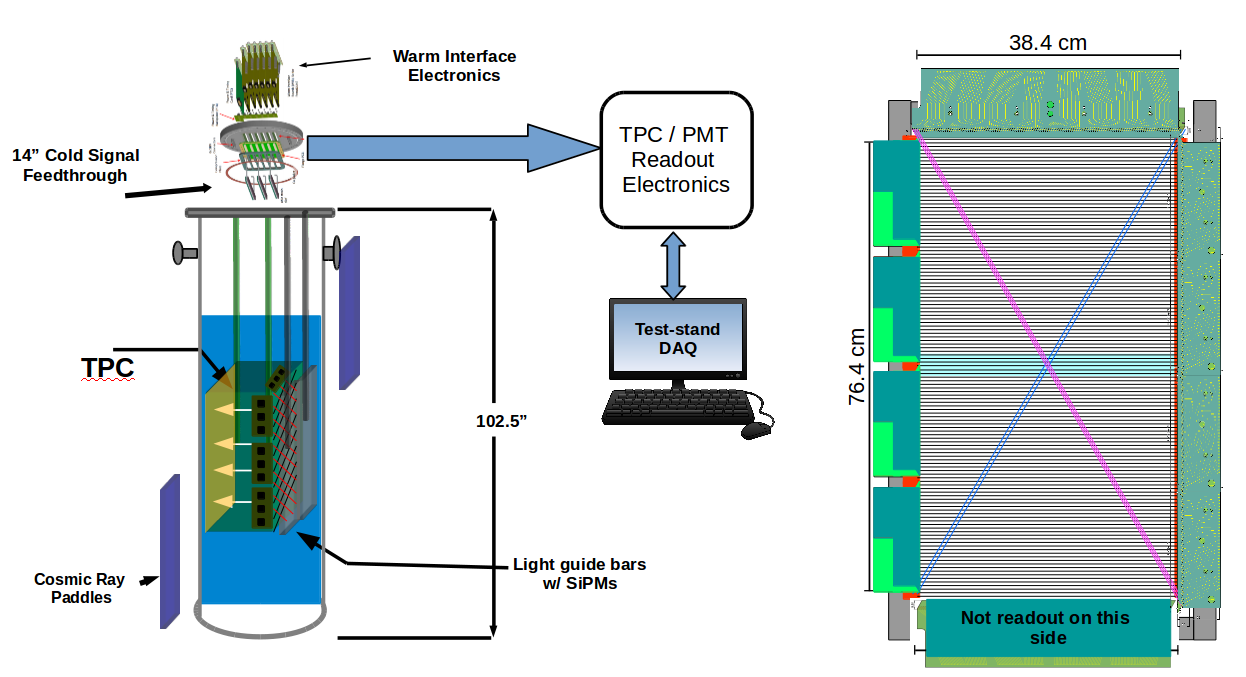
\includegraphics[width=0.68\textwidth]{images/teststand3.png}
\caption[]{Conceptual design of the SBND cold electronics vertical slice test-stand. Integration of both cold or warm electronics, light collection system, cosmic ray paddles, as well as warm interface electronics allows for complete testing of the entire readout system prior to deployment in the experiment and a platform for DAQ debugging outside the actual the experiment. The current design has 768 channels (256 collection, 512 induction) utilizing six SBND designed motherboards.}
\label{fig:teststand}
\end{figure} 

Inside this cryostat, a small scale TPC equipped with prototype cold readout electronics from SBND installed along side a pair of light guide bars can be deployed and readout through a 14'' inch cold signal feedthrough as designed for the SBND detector. External to the cryostat, scintillator paddles can be positioned to act as an external trigger. Since the cryostat is a copy of an existing one at FNAL, upon its completion the top flange and TPC detector will be shipped to FNAL for longer term use for SBND (and potentially other future LArTPCs). Additional material costs, such as the electronics, power supplies, and cabling are expected to be provided by SBND project funds and Prof. Asaadi's start-up funds.

This test-stand can allow for a robust set of tests for the integration of many new readout components prior to their deployment in the experiment. This critical step was not taken during the MicroBooNE assembly and as a result a number of problems with the readout electronics were not detected in advance of attempting to commission the detector. These problems included the bias voltage line for the TPC wires behaving in an unexpected way and causing pick-up noise to be seen on the electronics, cross-talk between the light detection system and the TPC readout, and the incorrect configuration of electronics settings because of software bugs. While many of these issues were able to be solved during the commissioning phase, they slowed the progress of transitioning to data taking and caused unnecessary harm to the experiment. Moreover, this test-stand will provide a platform for testing and debugging of the DAQ software and readout electronics configuration without interrupting the operation of the SBND experiment. 

The postdoctoral researcher and graduate student supported by this work will be developing the readout software into a common DAQ software package used by other LArTPC based experiments known as the artDAQ framework. This common platform ensures that the work done by those supported in this proposal can have a greater impact on future planned LArTPCs as well as allowing them to benefit from the work that has already been done by others.

Finally, such a test-stand can provide an R$\&$D platform for long term testing of future readout components as well as software development for online triggers and zero-suppression schemes without risking downtime on operating neutrino detectors. The trigger schemes envisioned include utilizing multi-core graphical processing units to do online TPC based triggering for rare search events such as proton decay and supernova neutrino triggering. Moreover, by providing a platform for the development of LArTPC's DAQ systems into a common platform such as artDAQ, a greater push to the integration of the data, simulation, and analysis into one common software platform can be accomplished. The events processed utilizing the artDAQ software are immediately readable by the common liquid argon software framework known as LArSoft. Thus, working on this system and the associated neutrino detectors DAQ help promote the use of a common software framework.


%%%%%%%%%%%%%%%%%%%%%%%%%%%%%%%%%%%%%%%%%%%%%%%%%%%%%%%%%%%%%%%%%%%%%
\subsection{Construction, Installation, and Commissioning}\label{sec:SBNDBulid}
%%%%%%%%%%%%%%%%%%%%%%%%%%%%%%%%%%%%%%%%%%%%%%%%%%%%%%%%%%%%%%%%%%%%%
The UT Arlington group is positioned to play a major role in the construction and commissioning of the SBND detector and data acquisition system. Given the groups experience from MicroBooNE and LArIAT (where Asaadi played a lead role of TPC expert during construction, commissioning, and operations for both experiments) as well as the experience of the post-doctoral researchers already with the group (Falcone from ICARUS and Chatterjee from LArIAT) UTA hopes to offer hands on leadership during the construction phase.

During the construction phase for the TPC (foreseen in mid 2017 through mid 2018), Falcone is expected to be in residence at FNAL and will be spending 50$\%$ of his time on SBND. During that same time, a to-be-named post-doc will join him at FNAL with a focus on SBND TPC construction. Having these two present will allow for a rapid ramp-up on the project. At the same time, the Cold-Electronics test-stand is expect to be moved from UTA to FNAL for operations. The graduate student Zach Williams is expected to go with this project in the summer of 2017 and be in residence at FNAL. With his time already spent on this project, continuing to contribute to the DAQ development and aiding in the construction and installation of the cold electronics on the TPC is a natural fit. PI Asaadi is expecting to spend a significant portion of his time at FNAL during the second half of 2017 to help oversee these activities and contribute to the construction and phase.

Following the construction and installation phase, one post-doc and one graduate student are expected to stay with the SBND experiment a significant portion of their time to play a role as detector experts during the commissioning and initial data taking. The aim here is to share their expertise across the SBN program, but to have a reliable source of experts in residence at FNAL for SBND. 





%%%%%%%%%%%%%%%%%%%%%%%%%%%%%%%%%%%%%%%%%%%%%%%%%%%%%%%%%%%%%%%%%%%%%
\subsection{SBND Data Analysis}\label{sec:SBNDDataAnalysis}
%%%%%%%%%%%%%%%%%%%%%%%%%%%%%%%%%%%%%%%%%%%%%%%%%%%%%%%%%%%%%%%%%%%%%
SBND will provide important physics measurements during its early operations in addition to providing an overall flux normalization to the key SBN oscillation analysis. Critically, SBND will collect very quickly statistics to confirm the nature of the MiniBooNE excess as measured by MicroBooNE. If MicroBooNE were to confirm the MiniBooNE excess as originating from electron-like sources, SBND could quickly measure if there is an oscillation component to the electron-like signal by measuring the rate as seen in the near detector. Conversely, if MicroBooNE were to determine the MiniBooNE excess as originating from photon-like sources, SBND can cross-check if the source is an unaccounted for beam like background or coming from cosmogenic like backgrounds. Regardless of the outcome, SBND will play a critical role in quickly collecting high statistics data as the near detector to the SBN program.

SBND will also provide critical neutrino cross-section measurements at a statistical precision unprecedented by any other LArTPC. SBND will collect approximately two million neutrino interactions per 2.2$\times 10^{20}$ protons  on target (roughly one year of running). With 1.5 million $\nu_{\mu}$ charged current interactions and 12,000 $\nu_{e}$ charged current interactions in one year. With such statistics, many precision cross-section measurements (e.g. double differential) become possible and improvements on first and second generation analyses from MicroBooNE can be explored in the first year of data taking.

Furthermore, by collecting approximately 100,000 NC$\pi^{0}$ events per year a full characterization of the leading background cross-section to the long baseline CP-violation analysis can be performed. The elimination of this systematic uncertainty in the cross-section will improve the experimental reach of the future planned DUNE experiment.
